% a mitges. La idea és fer una funció amb màxims, mínims i punts d'inflexió

\documentclass[tikz]{standalone}
\usepackage{pgfplots}
\pgfplotsset{compat=newest}
\pgfplotsset{plot coordinates/math parser=false}
\pgfplotsset{
    every non boxed x axis/.style={
        xtick align=center,
        enlarge x limits=true,
        x axis line style={line width=0.8pt, -latex}
},
    every boxed x axis/.style={}, enlargelimits=false
}
\pgfplotsset{
    every non boxed y axis/.style={
        ytick align=center,
        enlarge y limits=true,
        y axis line style={line width=0.8pt, -latex}
},
    every boxed y axis/.style={}, enlargelimits=false
}
\usetikzlibrary{
   arrows.meta,
  intersections,
}

\begin{document}

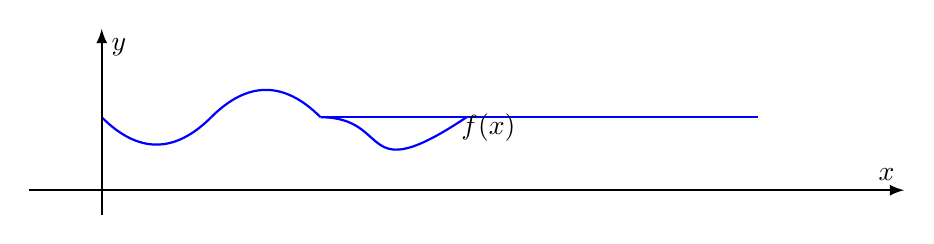
\begin{tikzpicture}
\begin{axis}[width=5in,axis equal image,
    axis lines=middle,
    xmin=0,xmax=20,
    xlabel=$x$,ylabel=$y$,
    ymin=-0.25,ymax=4,
    xtick={\empty},ytick={\empty}, axis on top
]

%
% \addplot[thick,domain=0.25:7,blue,name path = A]  {-x/3 + 2.75} coordinate[pos=0.4] (m) ;
\draw[thick,blue, name path =B] (0,2) .. controls (1,1) and (2,1) .. (3,2);
\draw[thick,blue, name path =B] (3,2) .. controls (4,3) and (5,3) .. (6,2);
\draw[thick,blue, name path =B] (6,2) .. controls (7,2) and (8,2) .. (9,2);
\draw[thick,blue, name path =B] (9,2) .. controls (10,2) and (11,2) .. (12,2);
\draw[thick,blue, name path =B] (12,2) .. controls (13,2) and (14,2) .. (15,2);
\draw[thick,blue, name path =B] (15,2) .. controls (16,2) and (17,2) .. (18,2);
\draw[thick,blue, name path =B] (6,2) .. controls (8,2) and (7,0) .. (10,2) node[pos=0.95, color=black, right]  {$f(x)$} coordinate[pos=0.075] (a1)  coordinate[pos=0.95] (a2);

% \path [name intersections={of=A and B, by={a,b}}];

%
% \draw[densely dashed] (0,0) -| node[pos=0.5, color=black, label=below:$a$] {}(a1);
% \draw[densely dashed] (0,0) -| node[pos=0.5, color=black, label=below:$x_{1}$] {}(a);
% \draw[ name path=D] (3,0) -|node[pos=0.5, color=black, label=below:$\lambda x_{1}+ (1-\lambda)x_{2}$] {} node[pos=1, fill,circle,inner sep=1pt] {}(m);
% \draw[densely dashed] (0,0) -|node[pos=0.5, color=black, label=below:$x_{2}$] {}(b);
% \draw[densely dashed] (0,0) -|node[pos=0.5, color=black, label=below:$b$] {}(a2);

% %
% \path [name intersections={of=B and D, by={c}}] node[fill,circle,inner sep=1pt] at (c) {};
%
% %
% \node[anchor=south west, text=black] (d) at (0.75,3) {$f[\lambda x_{1}+(1-\lambda)x_{2}]$};
% \node[anchor=south west, text=black] (e) at (3,2.5) {$\lambda f(x_{1})+(1-\lambda)f(x_{2})$};
% \draw[-{Latex[width=4pt,length=6pt]}] (d) -- (c);
% \draw[-{Latex[width=4pt,length=6pt]}] (e) -- (m);
\end{axis}
\end{tikzpicture}

\end{document}
